\begin{figure}
  \centering %
  \subfloat[\emph{Magni et al.\ }cascading binary model.]{%
    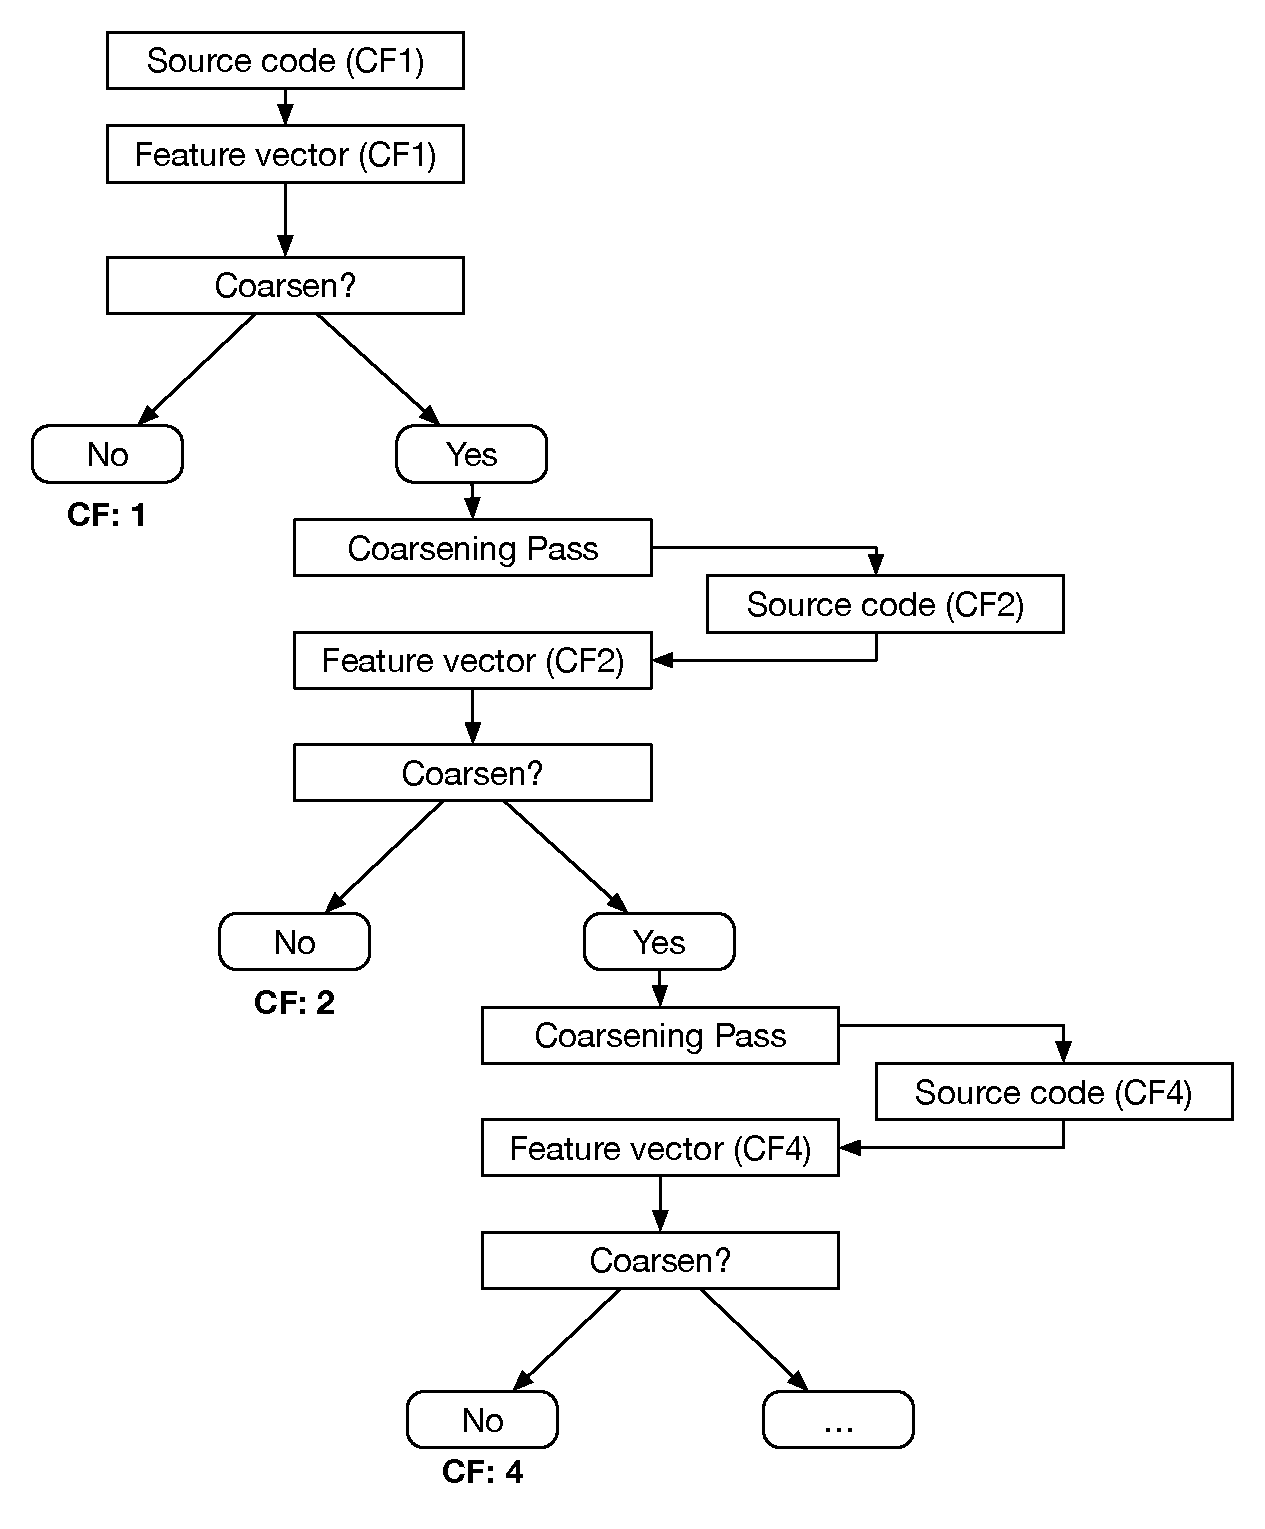
\includegraphics[width=.95\columnwidth]{img/cf-magni}%
    \label{fig:cf-magni}
  }\\*%
  \subfloat[Proposed approach.]{%
      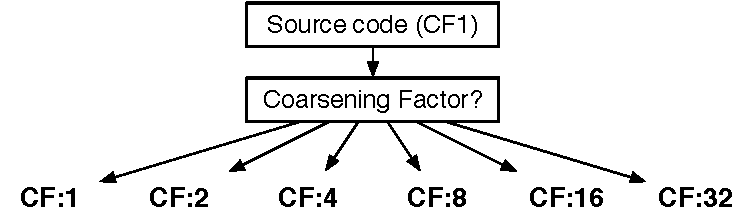
\includegraphics[width=.75\columnwidth]{img/cf-deeptune}%
      \label{fig:cf-deeptune}
  }%
  \caption[Predicting OpenCL thread coarsening factors.]{%
      Two approaches for predicting coarsening factor (CF) of OpenCL kernels.
      \emph{Magni et al.\ }reduce the multi-label classification problem to a
      series of binary decisions, by iteratively applying the optimisation and
      computing new feature vectors. Our approach simply predicts the coarsening
      factor directly from the source code.%
  }
  \label{fig:cascading-nn}
\end{figure}
